% Options for packages loaded elsewhere
\PassOptionsToPackage{unicode}{hyperref}
\PassOptionsToPackage{hyphens}{url}
\PassOptionsToPackage{dvipsnames,svgnames,x11names}{xcolor}
%
\documentclass[
  letterpaper,
]{report}

\usepackage{amsmath,amssymb}
\usepackage{iftex}
\ifPDFTeX
  \usepackage[T1]{fontenc}
  \usepackage[utf8]{inputenc}
  \usepackage{textcomp} % provide euro and other symbols
\else % if luatex or xetex
  \usepackage{unicode-math}
  \defaultfontfeatures{Scale=MatchLowercase}
  \defaultfontfeatures[\rmfamily]{Ligatures=TeX,Scale=1}
\fi
\usepackage{lmodern}
\ifPDFTeX\else  
    % xetex/luatex font selection
\fi
% Use upquote if available, for straight quotes in verbatim environments
\IfFileExists{upquote.sty}{\usepackage{upquote}}{}
\IfFileExists{microtype.sty}{% use microtype if available
  \usepackage[]{microtype}
  \UseMicrotypeSet[protrusion]{basicmath} % disable protrusion for tt fonts
}{}
\makeatletter
\@ifundefined{KOMAClassName}{% if non-KOMA class
  \IfFileExists{parskip.sty}{%
    \usepackage{parskip}
  }{% else
    \setlength{\parindent}{0pt}
    \setlength{\parskip}{6pt plus 2pt minus 1pt}}
}{% if KOMA class
  \KOMAoptions{parskip=half}}
\makeatother
\usepackage{xcolor}
\setlength{\emergencystretch}{3em} % prevent overfull lines
\setcounter{secnumdepth}{-\maxdimen} % remove section numbering
% Make \paragraph and \subparagraph free-standing
\ifx\paragraph\undefined\else
  \let\oldparagraph\paragraph
  \renewcommand{\paragraph}[1]{\oldparagraph{#1}\mbox{}}
\fi
\ifx\subparagraph\undefined\else
  \let\oldsubparagraph\subparagraph
  \renewcommand{\subparagraph}[1]{\oldsubparagraph{#1}\mbox{}}
\fi


\providecommand{\tightlist}{%
  \setlength{\itemsep}{0pt}\setlength{\parskip}{0pt}}\usepackage{longtable,booktabs,array}
\usepackage{calc} % for calculating minipage widths
% Correct order of tables after \paragraph or \subparagraph
\usepackage{etoolbox}
\makeatletter
\patchcmd\longtable{\par}{\if@noskipsec\mbox{}\fi\par}{}{}
\makeatother
% Allow footnotes in longtable head/foot
\IfFileExists{footnotehyper.sty}{\usepackage{footnotehyper}}{\usepackage{footnote}}
\makesavenoteenv{longtable}
\usepackage{graphicx}
\makeatletter
\def\maxwidth{\ifdim\Gin@nat@width>\linewidth\linewidth\else\Gin@nat@width\fi}
\def\maxheight{\ifdim\Gin@nat@height>\textheight\textheight\else\Gin@nat@height\fi}
\makeatother
% Scale images if necessary, so that they will not overflow the page
% margins by default, and it is still possible to overwrite the defaults
% using explicit options in \includegraphics[width, height, ...]{}
\setkeys{Gin}{width=\maxwidth,height=\maxheight,keepaspectratio}
% Set default figure placement to htbp
\makeatletter
\def\fps@figure{htbp}
\makeatother

\usepackage{titling}
\pretitle{
  \begin{center}
  \huge
  
\includegraphics[width=4cm,height=6cm]{psulogo2.jpg}\\[\bigskipamount]
}
\posttitle{\end{center}}
\posttitle{\end{center}}
\usepackage{booktabs}
\usepackage{longtable}
\usepackage{array}
\usepackage{multirow}
\usepackage{wrapfig}
\usepackage{float}
\usepackage{colortbl}
\usepackage{pdflscape}
\usepackage{tabu}
\usepackage{threeparttable}
\usepackage{xcolor}
\usepackage{soul}
\usepackage{graphicx}
\usepackage{fancyhdr}
\pagestyle{fancy}
\rhead{
\includegraphics[width = .05\textwidth]{psulogo2.jpg}}
\makeatletter
\makeatother
\makeatletter
\makeatother
\makeatletter
\@ifpackageloaded{caption}{}{\usepackage{caption}}
\AtBeginDocument{%
\ifdefined\contentsname
  \renewcommand*\contentsname{Table of contents}
\else
  \newcommand\contentsname{Table of contents}
\fi
\ifdefined\listfigurename
  \renewcommand*\listfigurename{List of Figures}
\else
  \newcommand\listfigurename{List of Figures}
\fi
\ifdefined\listtablename
  \renewcommand*\listtablename{List of Tables}
\else
  \newcommand\listtablename{List of Tables}
\fi
\ifdefined\figurename
  \renewcommand*\figurename{Figure}
\else
  \newcommand\figurename{Figure}
\fi
\ifdefined\tablename
  \renewcommand*\tablename{Table}
\else
  \newcommand\tablename{Table}
\fi
}
\@ifpackageloaded{float}{}{\usepackage{float}}
\floatstyle{ruled}
\@ifundefined{c@chapter}{\newfloat{codelisting}{h}{lop}}{\newfloat{codelisting}{h}{lop}[chapter]}
\floatname{codelisting}{Listing}
\newcommand*\listoflistings{\listof{codelisting}{List of Listings}}
\makeatother
\makeatletter
\@ifpackageloaded{caption}{}{\usepackage{caption}}
\@ifpackageloaded{subcaption}{}{\usepackage{subcaption}}
\makeatother
\makeatletter
\@ifpackageloaded{tcolorbox}{}{\usepackage[skins,breakable]{tcolorbox}}
\makeatother
\makeatletter
\@ifundefined{shadecolor}{\definecolor{shadecolor}{rgb}{.97, .97, .97}}
\makeatother
\makeatletter
\makeatother
\makeatletter
\makeatother
\ifLuaTeX
  \usepackage{selnolig}  % disable illegal ligatures
\fi
\usepackage[]{biblatex}
\addbibresource{references.bib}
\IfFileExists{bookmark.sty}{\usepackage{bookmark}}{\usepackage{hyperref}}
\IfFileExists{xurl.sty}{\usepackage{xurl}}{} % add URL line breaks if available
\urlstyle{same} % disable monospaced font for URLs
\hypersetup{
  pdftitle={Separating intended versus unintended learning effect in implicit learning with preschoolers},
  pdfauthor={Elizabeth (``Betsy'') Camp; Ryan Masson; Will McIntosh; Lauren Montefalcon},
  colorlinks=true,
  linkcolor={blue},
  filecolor={Maroon},
  citecolor={Blue},
  urlcolor={Blue},
  pdfcreator={LaTeX via pandoc}}

\title{Separating intended versus unintended learning effect in implicit
learning with preschoolers}
\usepackage{etoolbox}
\makeatletter
\providecommand{\subtitle}[1]{% add subtitle to \maketitle
  \apptocmd{\@title}{\par {\large #1 \par}}{}{}
}
\makeatother
\subtitle{CADES Consulting Lab}
\author{Elizabeth (``Betsy'') Camp \and Ryan Masson \and Will
McIntosh \and Lauren Montefalcon}
\date{2023-05-14}

\begin{document}
\maketitle
\ifdefined\Shaded\renewenvironment{Shaded}{\begin{tcolorbox}[enhanced, interior hidden, frame hidden, boxrule=0pt, sharp corners, breakable, borderline west={3pt}{0pt}{shadecolor}]}{\end{tcolorbox}}\fi

\renewcommand*\contentsname{Table of contents}
{
\hypersetup{linkcolor=}
\setcounter{tocdepth}{2}
\tableofcontents
}
\newpage{}

\hypertarget{executive-summary}{%
\section{Executive Summary}\label{executive-summary}}

The primary goal of the work described herein is to separate out the
impact of an alternating visual cue from the intended learning effect of
an auditory cue on a participants response in experimental data on
implicit learning in preschoolers. Multiple analysis approaches were
considered which culminated in moving toward causal inference approaches
often seen in longitudinal studies in medicine where time-varying
confounders are commonplace. Our current recommendation to pursue two
analysis methods which differ from one another but seem most likely to
be successful in achieving the goal of separating the impact of the
confounding visual cue as well as both being feasible to execute from a
technical perspective.

\hypertarget{introduction-and-background}{%
\section{Introduction and
Background}\label{introduction-and-background}}

An experimental study was done comparing implicit learning of
preschoolers with developmental language disorder (DLD) versus
preschoolers with typical language development (TLD). Participants were
first tested on their ability to differentiate between the auditory cues
that would be used in the subsequent parts of the experiment. Then,
participants underwent a computer-based ``training'' period where a
``monster'' on the computer screen asked for food or drink by emitting
sounds of a specific pitch or duration. In other words, participants
were given an auditory cue in the form of a sound with a pitch or
duration, which was associated with a specific visual cue in the form of
an image of food or drink. Participants would press keys on the computer
keyboard either before or after the image appeared to indicate whether
food or drink was being requested based on the sound emitted by the
monster. In the testing phase of the experiment, participants were
exposed to the sound, and they indicated on the keyboard whether the
monster was asking for food or drink. Only after the participant entered
their response on the keyboard did the image of the food or drink appear
on the computer screen. Note that in both training and testing phases,
the image of the drink would appear from the left-hand side of the
screen and the image of food would appear from the right. The order of
the food or drink trials were pseudo-random. However, in the process of
psuedo-randomizing, the food and drink typically alternated. This
alternation allowed participants to formulate a heuristic to predict
whether the next trial would be food or drink based on the present
trial. Figure 1 shows a visual depiction of both training and testing
phases of the experiment.

\begin{figure}

{\centering 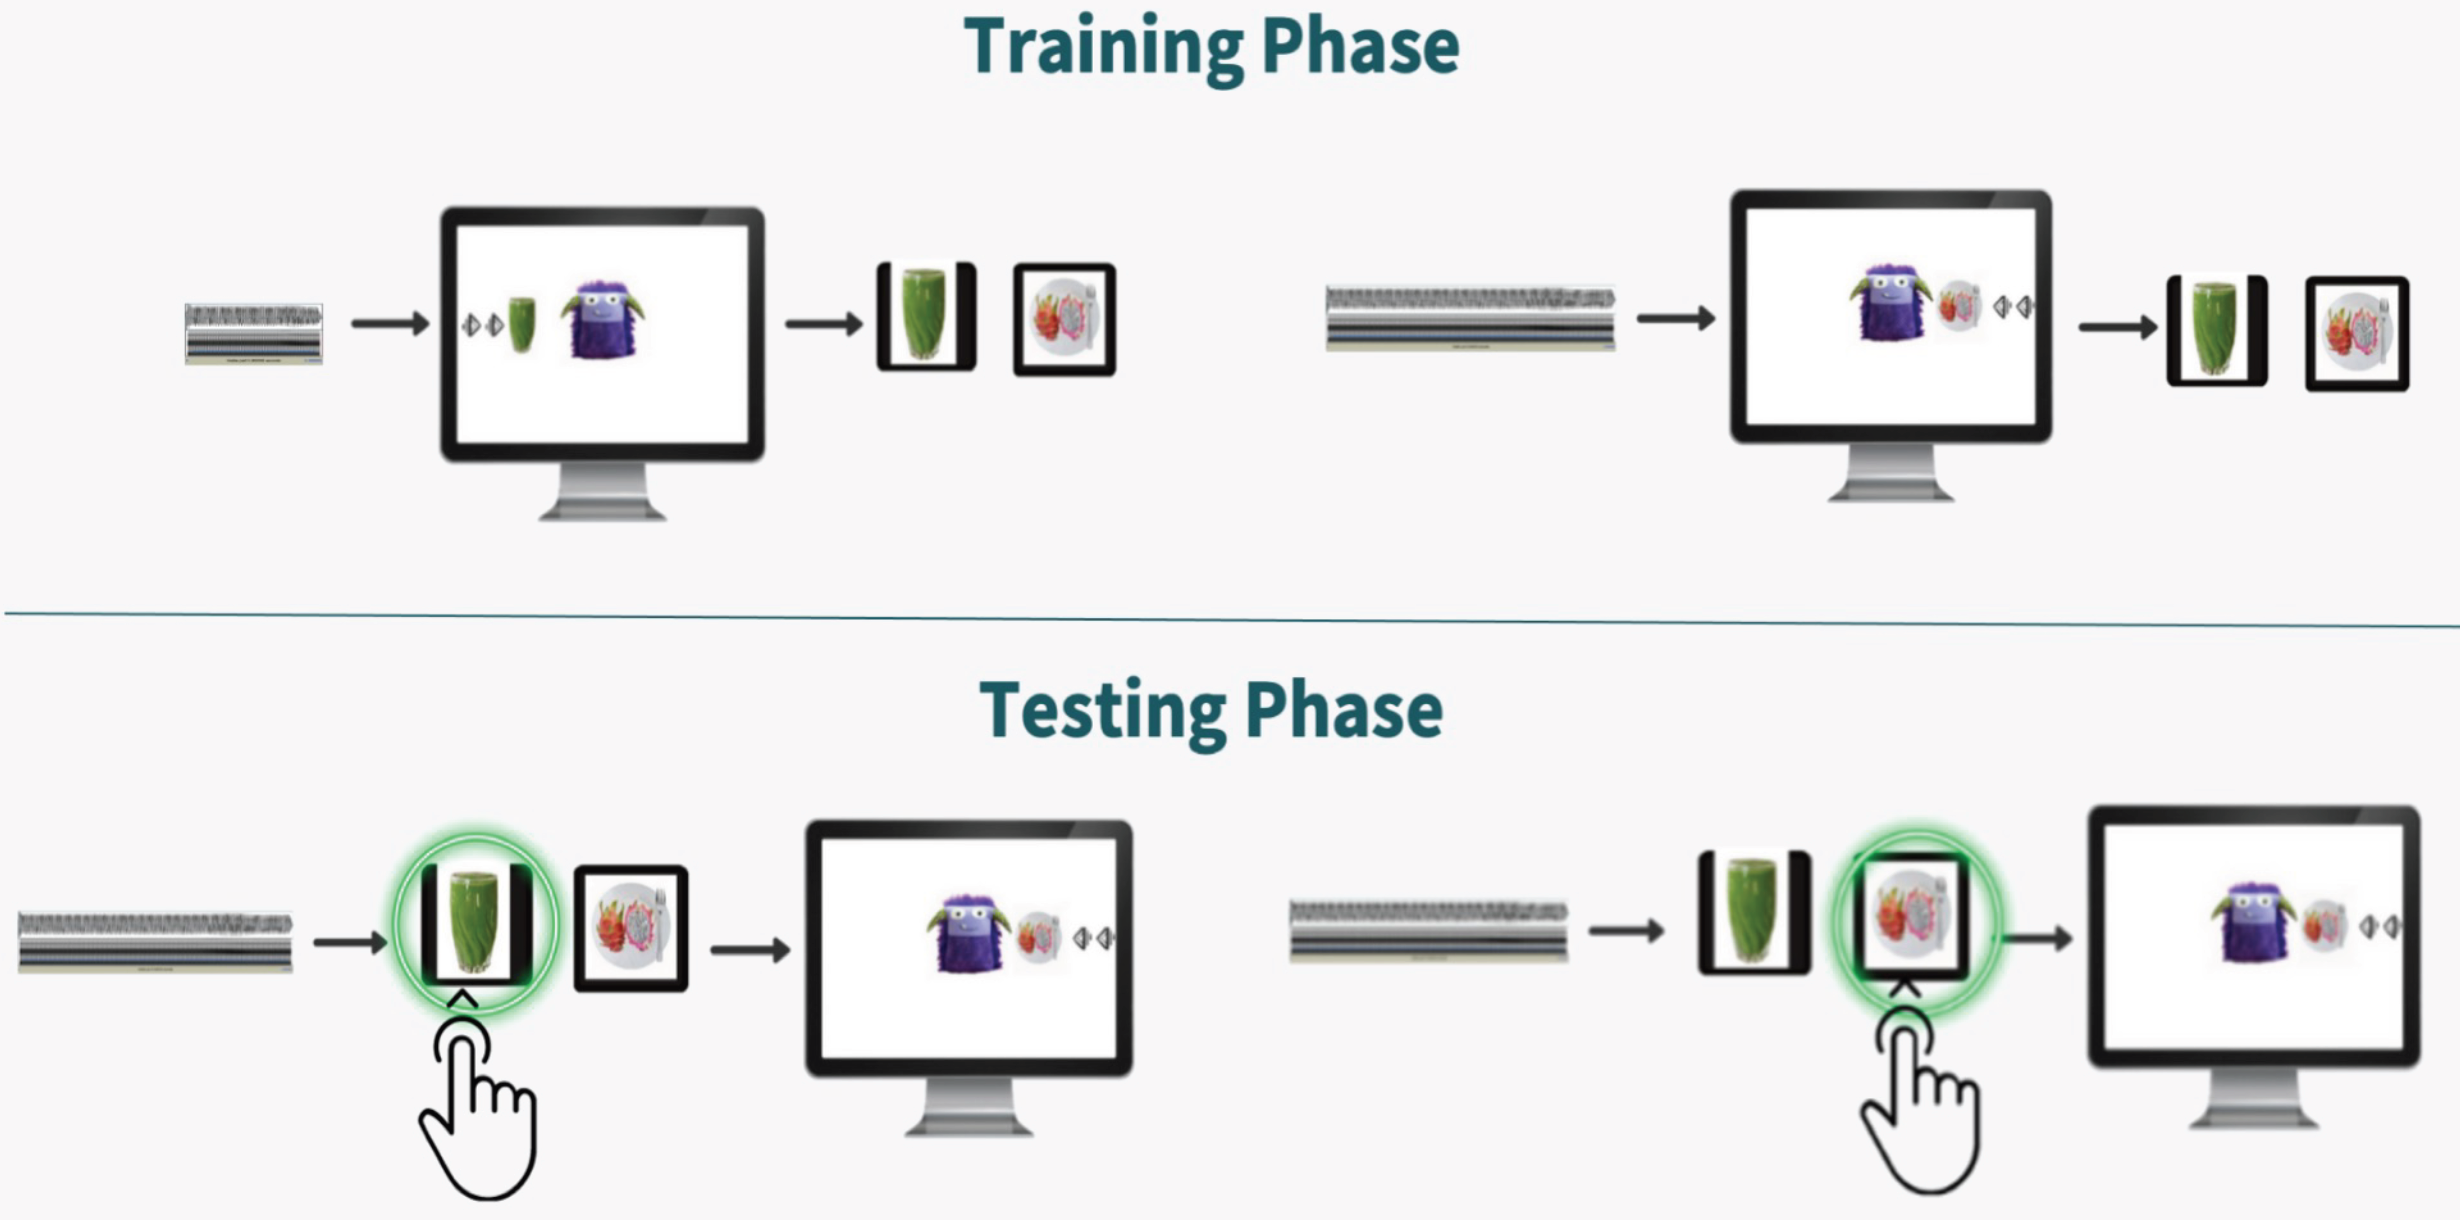
\includegraphics[width=0.9\textwidth,height=\textheight]{../../visualization/preschoolers_exp_setup.png}

}

\caption{Experimental set up of the traing and testing phase showing
sound which varies in pitch or duration which is associate with either
food or drink (reprinted from
\textcite{cairns_crystal_l_implicit_2022}).}

\end{figure}

Due to the frequent alternation of food and drink and the associated
heuristic, participants adopted to predict whether food or drink be
indicated in the subsequent trial, the experimental results show a
combined learning effect. Specifically, the experimental results contain
both the effect of the learned alternation heuristic with the learned
association of a sound with the food or drink.

The goal of the work herein was to determine if the learned alternation
heuristic could be separated from the learned sound and food/drink
association.

\hypertarget{data}{%
\section{Data}\label{data}}

\hypertarget{basic-data-description}{%
\subsection{Basic Data Description}\label{basic-data-description}}

The experimental results utilized in the present work were in tabular
form. The response variable shows whether the participant was correct or
incorrect in indicating whether the monster requested food or drink.
Thus, the response variable has a binary form. Additional variables
explored were response time in seconds, trial number, trial order type,
sound type, experimental phase (training, testing), alternation from
previous trial, and participant type (TLD, DLD). There were 26
participants with DLD and 26 participants in the TLD class. Participant
data such as school test scores were recoded in order to ensure
participants' identifiable information remained confidential.

\hypertarget{exploratory-data-analysis}{%
\subsection{Exploratory Data Analysis}\label{exploratory-data-analysis}}

Since the fundamental goal herein is to separate the alternation on the
response variable from any learned association between the pitch or
duration of the sound and the food/drink, the number of participants in
each class was first examined. Figure 2 shows the count of participants
with DLD versus TLD in each trial order group. The trial order group
specifies the sequence of alternation of the stimuli in the training and
tests.

\begin{figure}

{\centering 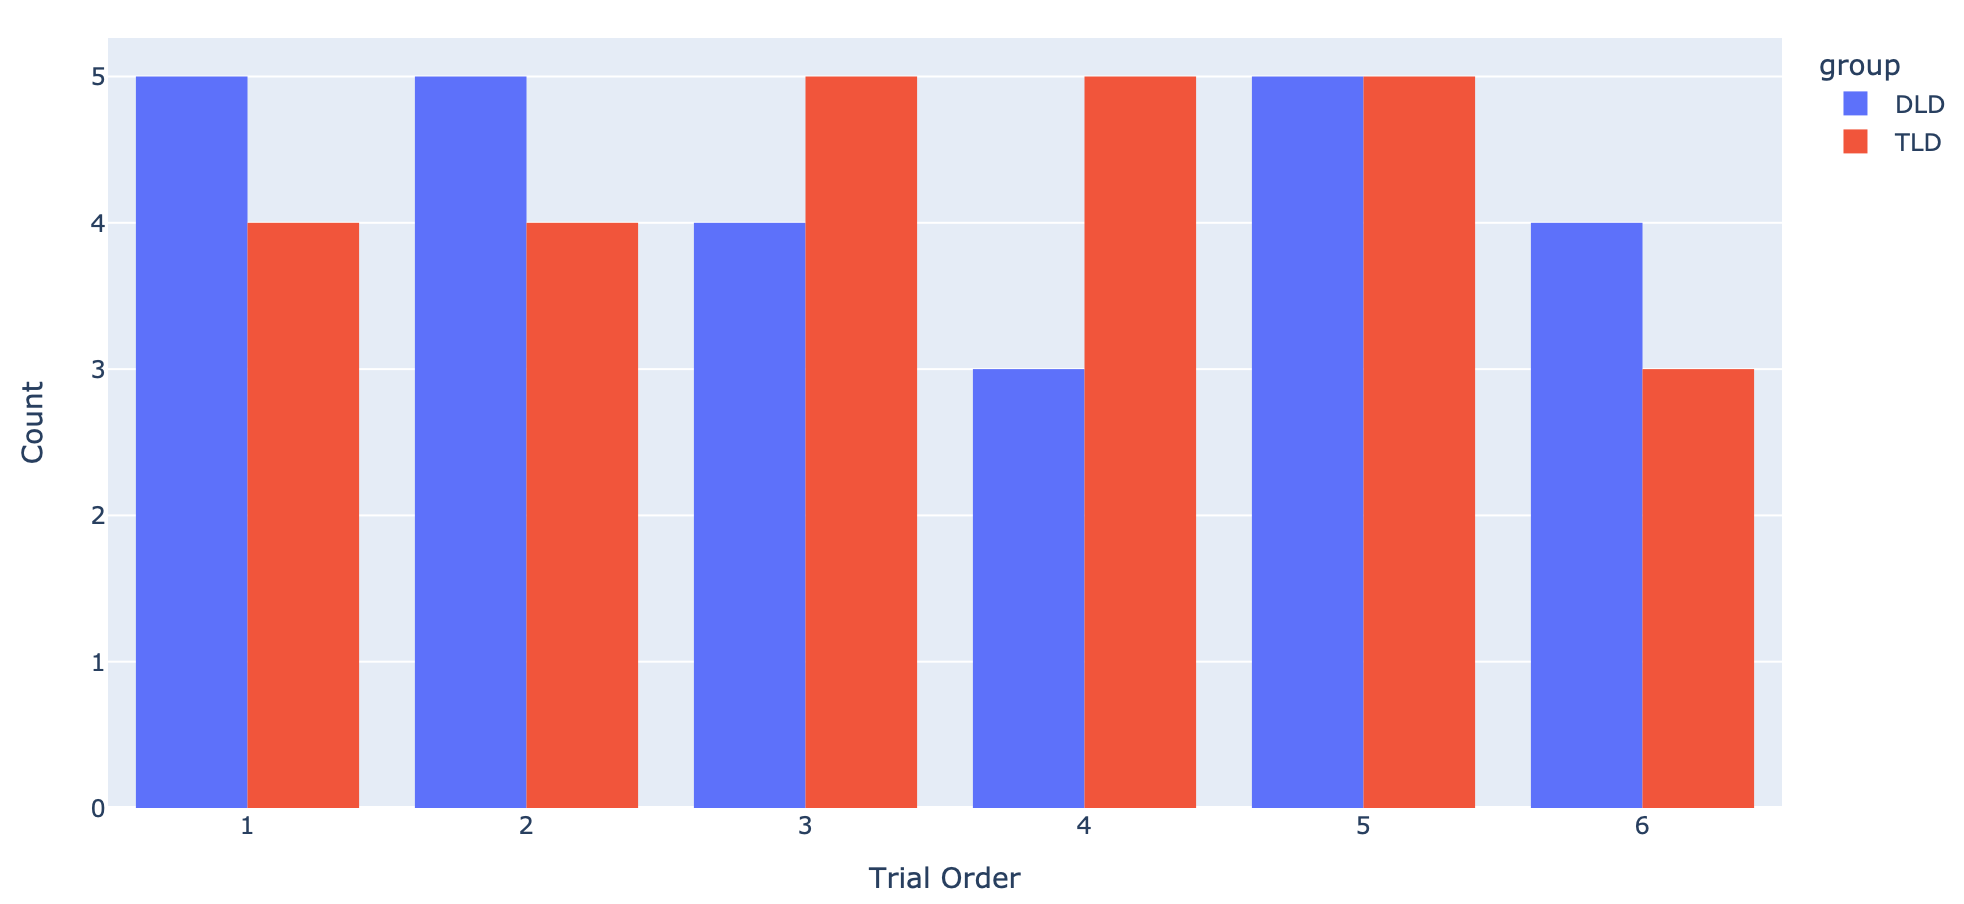
\includegraphics[width=0.9\textwidth,height=\textheight]{../../visualization/count_trialorder_participants.png}

}

\caption{Count of participants in each trial order with DLD versus TLD}

\end{figure}

In Figure 2, the count of participants in each trial order group with
DLD or TLD varies between 3 and 5. Thus, the number of participants in
each class is not perfectly balanced. This small imbalance in
participants will impact any subsequent analysis conditioned on TLD/DLD
and trial order. Note that the count of participants with TLD versus
those with DLD is perfectly balanced, with both counts being 26.

The response variable for each trial is whether the keyboard entry by
the participant correctly or incorrectly indicates whether food or drink
was called for by the monster's sounds. However, the response time for
the participant's keyboard entry does suggest something about how the
participant is learning during the training or testing phases. Figure 3
shows the participant response time in seconds as a function of the
trial number during the training phase of the experiment. Data for
participants with DLD versus TLD are shown by different marker colors in
Figure 3, and a linear fit through the DLD versus TLD groups is
superimposed on the response time. Figure 4 shows the corresponding data
for response time as a function of the trial number for the testing
phase of the experiment. Note that the ordinary least squares linear fit
is shown for convenience to obtain a visual indicator of key trends. In
order to make statements as to whether differences in slopes are
statistically significant, hypothesis testing should be performed. For
example, if the slope of the linear fit of the DLD participants during
training is \(\beta_{1,train}\) and the slope of the linear fit of the
DLD participants during testing is \(\beta_{1,test}\), we could test the
null hypothesis of \(\beta_{1,train}=\beta_{1,test}\) versus
\(\beta_{1,train} \neq \beta_{1,test}\) to determine if the slopes are
significantly different.

\begin{figure}

{\centering 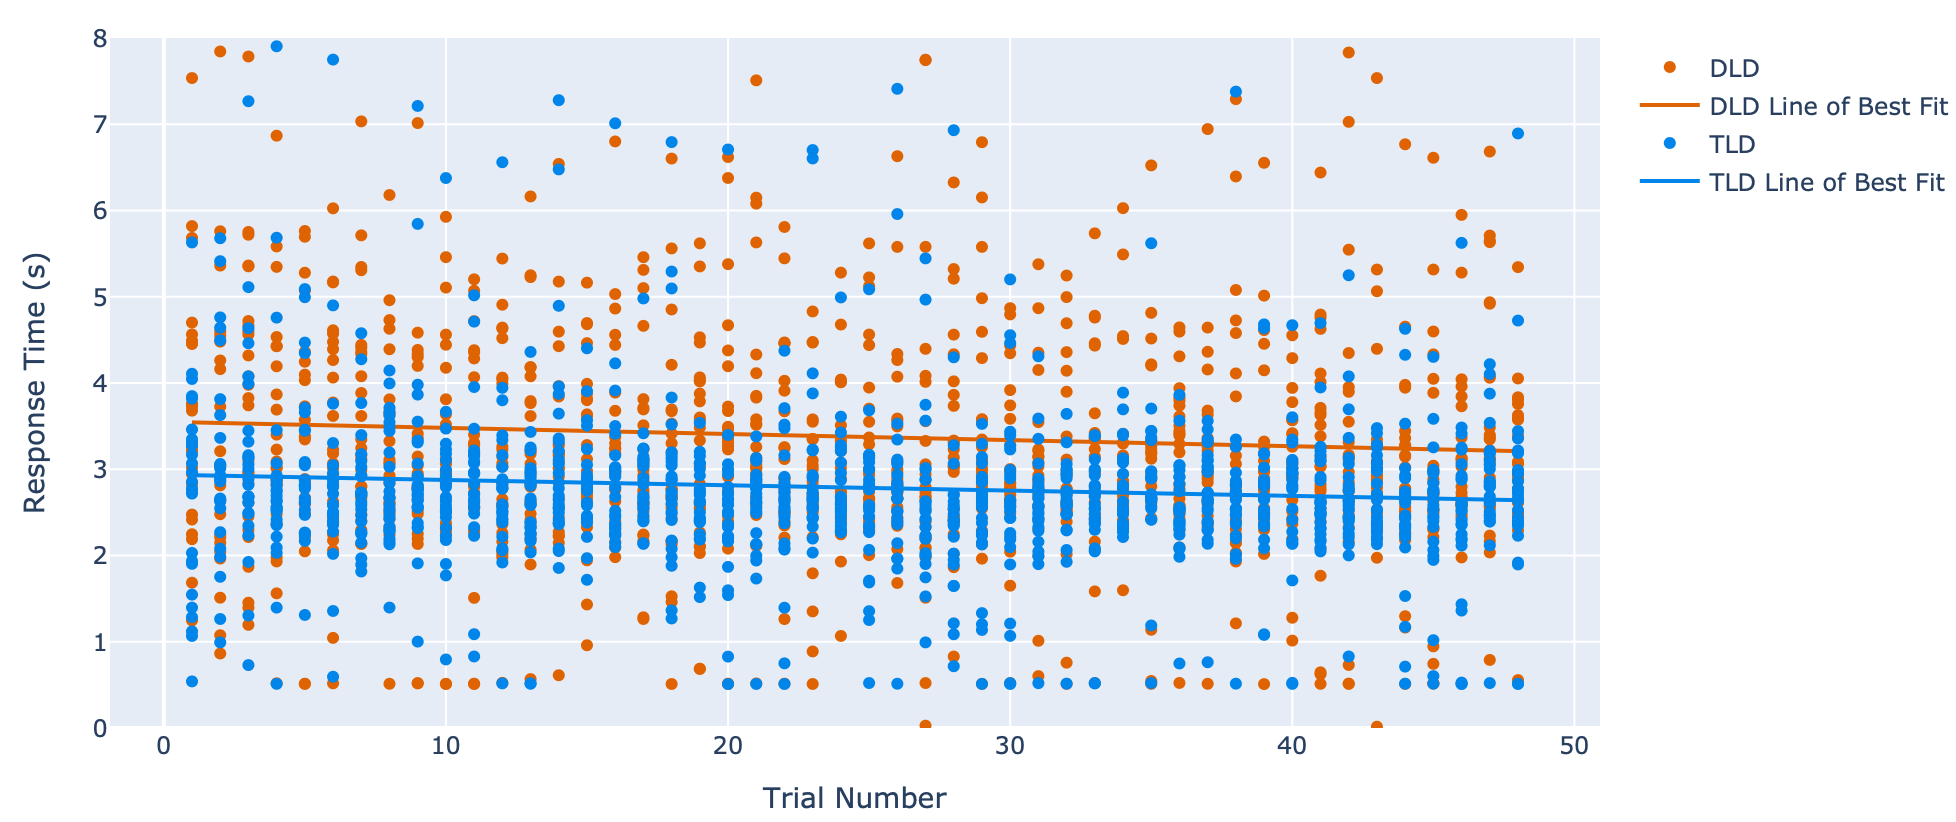
\includegraphics[width=0.9\textwidth,height=\textheight]{../../visualization/response_time_training.png}

}

\caption{Response time as a function of trial number during training
phase}

\end{figure}

Surprisingly, the slope of the linear fit in the training period (see
Figure 3) is smaller than in the testing period (see Figure 4),
particularly for the DLD participants. This response time change
suggests that the participants' interaction with the stimuli and, thus,
any learning is perhaps still occurring during the testing phase of the
experiment. We expected different sets of trends in Figures 3 and 4.
Specifically, we expected that the response time would change more in
the training phase than the testing phase and we expected a relatively
minor change in response time during the testing phase. Furthermore, we
expected the response time to change more for TLD versus DLD
participants if the TLD participants learned at a greater rate than DLD
participants.

\begin{figure}

{\centering 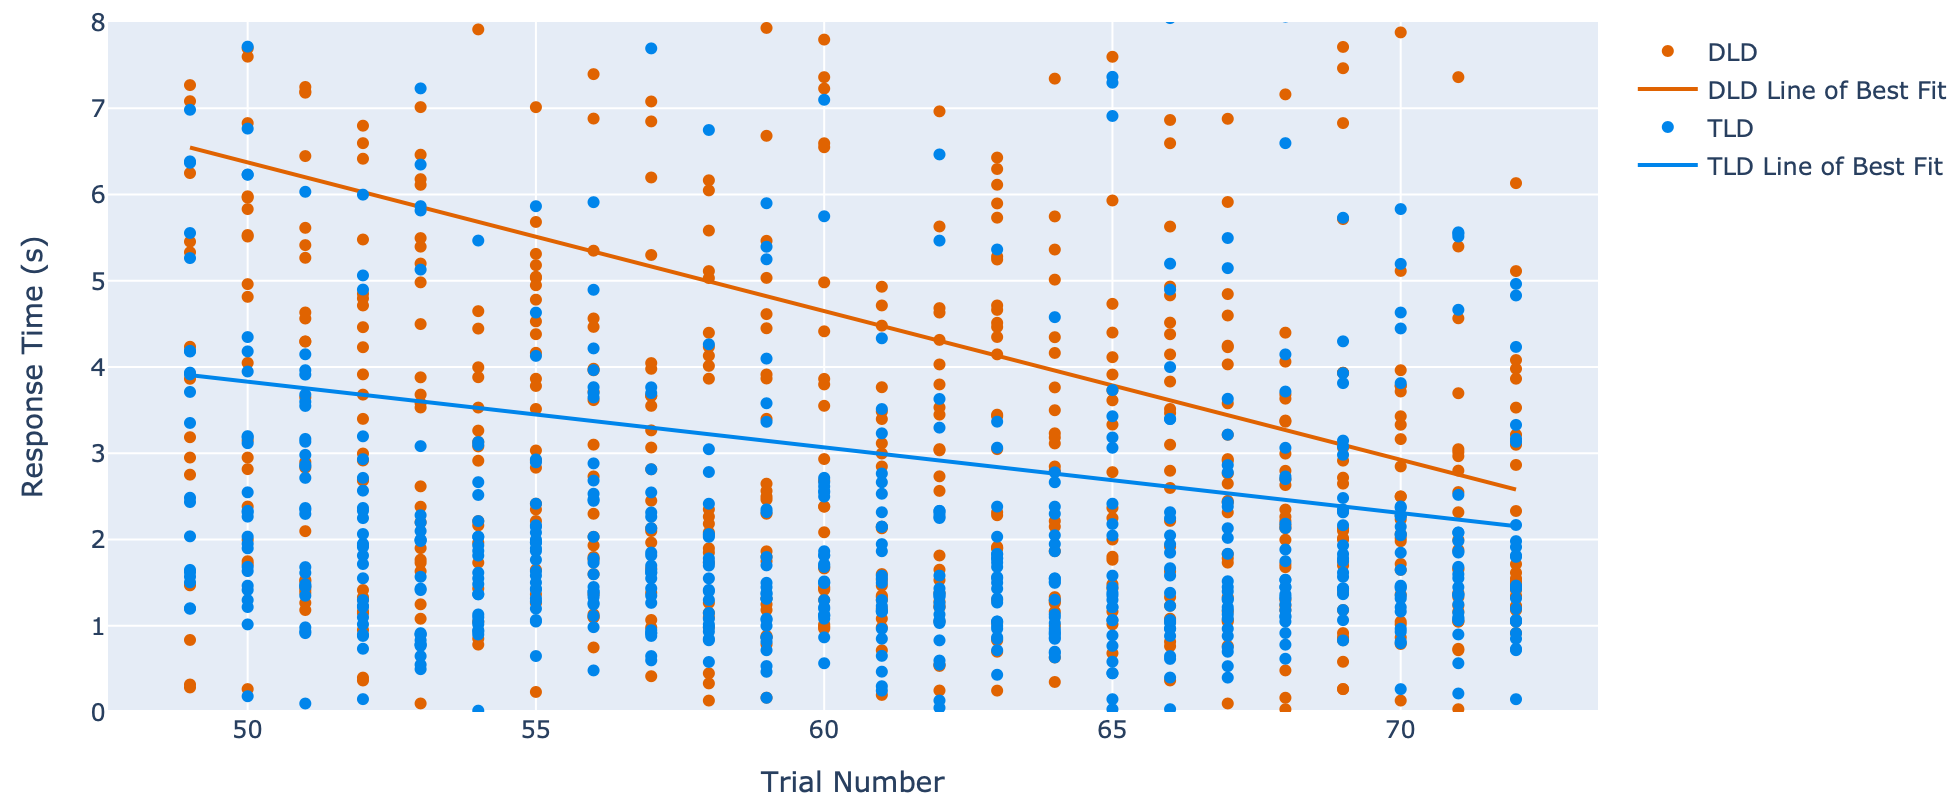
\includegraphics[width=0.9\textwidth,height=\textheight]{../../visualization/response_time_testingphase.png}

}

\caption{Response time as a function of trial number during testing
phase}

\end{figure}

\hypertarget{connect-the-dots-eda}{%
\section{Connect the dots: EDA}\label{connect-the-dots-eda}}

Analysis methods aimed at isolating the impact of the visual alternation
of food/drink from the impact of the sound on the participant's keyboard
response typically involve conditioning on the alternation indicator
variable and the sound variable. The number of participants in each
trial order class is not perfectly balanced, which may reduce our
ability to detect differences. Furthermore, one analysis approach would
be to conceive of the trials as individual treatment periods in a
cross-over experimental design. The fact that the response time changes
as a function of the trial number indicates an interaction from period
to period which would increase Type I error in an analysis of this type
(see Methods section for further information).

\hypertarget{methods}{%
\section{Methods}\label{methods}}

\hypertarget{methods-examined-and-determined-unsuitable}{%
\subsection{Methods examined and determined
unsuitable}\label{methods-examined-and-determined-unsuitable}}

First, we explored separating the audio learning cue from the unintended
visual cue as a process of fitting a mixed effects model based on a
crossover experimental design. This seemed to be a promising approach
that might allow us to estimate the effect of the visual cue on the
testing accuracy of the children, and thus control for it.

A mixed effects model based on conceptualizing each trial of the present
experiment as a period in a crossover design initially seemed like a
good choice. In a crossover experimental design, the study involves
sequences of treatments applied to individual subjects over successive
time periods. In this type of experiment, the individual participant
becomes a random effect due to the study participants being a sample
from the theoretical larger populations of children with DLD and TLD. So
a mixed effects model could include the fixed effect of the implicit
learning treatment (the sound files), the random effect of the
participant, and the fixed effect of the alternation pattern.

We did note that there are inherent difficulties with approaching this
study as a crossover design. One of the critical challenges in a
crossover design can arise when a treatment effect from one period is
still present in subsequent periods. A treatment effect that persists
from one period to later periods is called a carryover effect. In the
present study, carryover effects would be present if learning from one
trial impacted the next or subsequent trials. In Figure 4, we observed
that response times in the testing trials decreased over the course of
the testing phase, suggesting that the participants were continuing to
learn during the trials in the testing phase. Due to the carryover
effects that appear to be present between subsequent trials in the
testing phase of the experiment, we concluded that analyzing the
experimental data as if it was a crossover experimental design would not
be suitable (see \textcite{noauthor_lesson_nodate}).

Another approach we considered was to fit mixed effects model with
additional lag terms. We envisioned that lag terms would capture the
alternation from previous trials that could potentially impact the
present trial under consideration. For example, one such model with lag
terms would be

\begin{equation}\protect\hypertarget{eq-mixed-effects-lagterm}{}{
y_t = f(group, soundDim_t, soundLevel_t , trialOrder, trial, side_{t-1})
}\label{eq-mixed-effects-lagterm}\end{equation}

where \(y_t\) is the response of correct or incorrect for trial \(t\),
group is the language development group TLD or DLD, \(soundDim_t\) is
pitch or duration for trial \(t\), \(soundLevel_t\) is the pitch or
duration level of trial \(t\), \(trialOrder\) is the participant trial
order group which describes the sequence of food or drink, \(trial\) is
the trial number, and \(side_{t-1}\) describes whether the side
alternated in the previous trial. We investigated using the
\texttt{gam()} function from the R package \texttt{mgcv} to fit a mixed
effects model similar to Equation~\ref{eq-mixed-effects-lagterm} and was
implemented by Simpson \emph{et al.} (\textcite{simpson_using_2021}).
However, we determined that another approach was needed because the
treatment is time-varying and the confounding due to side alternation is
also time-varying which cannot be handled adequately in this method.

\hypertarget{methods-for-further-consideration}{%
\subsection{Methods for further
consideration}\label{methods-for-further-consideration}}

Time-varying treatment and time-varying confounding are sometimes
present in longitudinal studies common in medicine. As a result, various
methods have been developed to analyze such studies, including causal
inference methods. Three causal inference methods were considered,
including the G-formula method, inverse probability weighting, and
G-estimation. Of these, the G-formula approach seems most appropriate
and feasible since an R package has been developed to implement this
method (\textcite{mcgrath_gformula_2020}), and interactions between the
time-varying treatment and time-varying covariates can be explored and
are explicitly modeled (\textcite{daniel_methods_2013}). Furthermore,
both binary and continuous response variables can be handled, allowing
the method to be applied to each trial or collectively to estimate a
total effect (\textcite{daniel_methods_2013}).

In addition to causal inference methods, another approach that has been
used for longitudinal studies with time-varying treatments and
time-varying covariates in the literature is sequential conditional mean
models (SCMM) fitted using generalized estimating equations (GEEs)
(\textcite{keogh_analysis_2018}). While the seminal work on the use of
SCMMs fitted using GEEs was published in 2018, the approach has been
applied by Beccia et al., wherein an appropriate R package to carry out
modeling using the SCMM fitted using a GEE was identified
(\textcite{beccia_cumulative_2022}). One of the advantages of SCMMs is
that these models are essentially standard regression models with
multiple additional terms reflecting past treatment exposure as well as
exposure to the time-varying covariate(s). Furthermore, SCMMs are also
adjusted via propensity score to improve robustness. The propensity
score of a participant at time \(t\) is the participant's probability of
having the treatment exposure at time \(t\) conditioned on experimental
conditions at all previous time points.

The open-source package gfoRmula, released in 2020, implements the
G-formula
(https://www.cell.com/patterns/fulltext/S2666-3899(20)30008-8). Adapting
the package to the language development study primarily involves
defining the output type as well as the input data frame. The likely
best outcome type to use is ``continuous end of follow-up,'' using each
participant's accuracy score at the end of the testing period as the
response variable. Then an input data frame to the main gformula()
function must be defined, as shown in the below figure. We would then
take coefficient estimates from the resulting models and interpret the
effect of alternation on participant accuracy.

\begin{figure}

{\centering 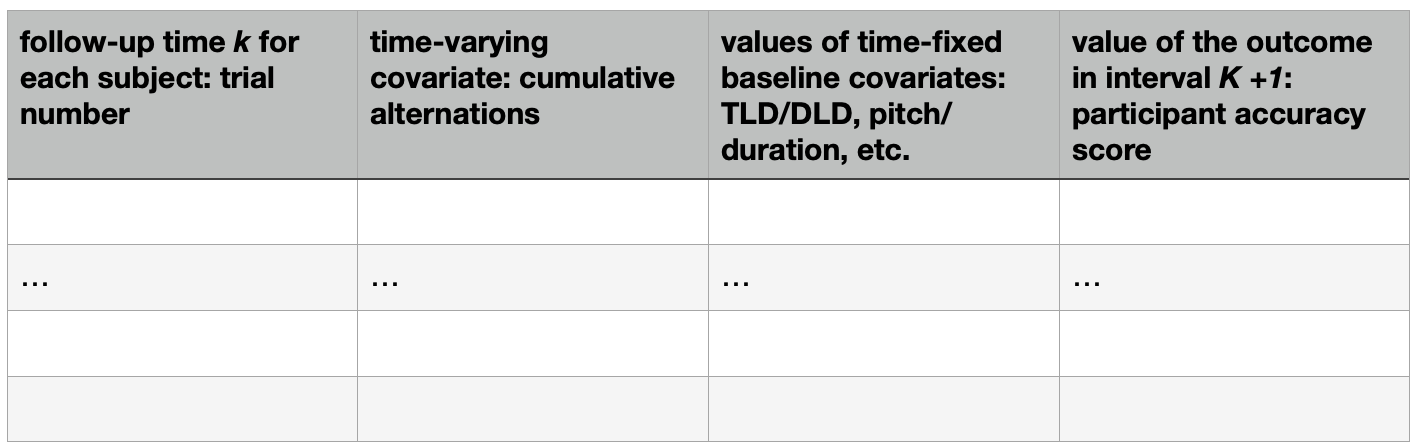
\includegraphics[width=0.9\textwidth,height=\textheight]{../../visualization/gformula_dataframe.png}

}

\caption{Outline of input data frame to gformula(); header is in the
format ``column definition from the package release: adaptation to the
language development study''}

\end{figure}

\hypertarget{conclusions-and-recommendations}{%
\section{Conclusions and
Recommendations}\label{conclusions-and-recommendations}}

Separating the effect of an auditory cue from an unintended alternating
visual cue is a challenging problem. The experimental data has been
explored and characterized. Analysis methods were identified and
ultimately discarded. Two promising approaches, the G-formula method and
sequential conditional mean models (SCMM), have been identified, which
have been successfully applied in the literature. These methods have
been used advantageously in studies with time-varying treatments and
time-varying covariates. In the present experiment, the time-varying
treatment is the combined sound type (pitch or duration) with the level
of the sound, and the time-varying covariate is the impact of the
alternating visual cue. The G-formula method and SCMMs seem technically
feasible, and R packages have been found to enable the execution of both
approaches. We recommend that both methods be pursued in future work.

\printbibliography[heading=none]




\end{document}
